\RequirePackage{amsthm} %https://tex.stackexchange.com/questions/687324/unknown-theoremstyle-warning-with-springer-nature-template
\documentclass[sn-mathphys-num,iicol]{sn-jnl}

%\usepackage{sn-jnl.sty}
\usepackage{graphicx}%
\usepackage{multirow}%
\usepackage{amsmath,amssymb,amsfonts}%
\usepackage{amsthm}%
\usepackage{physics}
\usepackage{siunitx}
\usepackage{mathrsfs}%
\usepackage[title]{appendix}%
\usepackage{xcolor}%
\usepackage{textcomp}%
\usepackage{manyfoot}%
\usepackage{booktabs}%
\usepackage{algorithm}%
\usepackage{algorithmicx}%
\usepackage{algpseudocode}%
\usepackage{listings}%
\usepackage{newtxmath}%
\usepackage[tiny]{titlesec}%
\usepackage[ngerman]{babel}
\usepackage{booktabs}

\theoremstyle{thmstyleone}
\newtheorem{theorem}{Theorem}
\newtheorem{proposition}[theorem]{Proposition}

\theoremstyle{thmstyletwo}
\newtheorem{remark}{Remark}

\theoremstyle{thmstylethree}
\newtheorem{definition}{Definition}

\raggedbottom

\newcommand{\td}{\text{d}}

\titleformat{\subsection}{}{\thesubsection}{1em}{\itshape}
\titleformat{\subsubsection}{}{\thesubsubsection}{1em}{\itshape}

\begin{document}
        
\title[]{Praktikum 4 -- Versuch 422: Rastertunnelmikroskop}
\author*[1]{\fnm{Jonas} \sur{Wortmann}}\email{s02jwort@uni-bonn.de}
\author*[2]{\fnm{Angelo} \sur{Brade}}\email{s72abrad@uni-bonn.de}
\affil*[1,2]{Rheinische Friedrich--Wilhelms--Universität, Bonn}

\maketitle

\section{Einleitung}
Wenn sich zwei leitende Materialien mit verschiedenen Austrittsarbeiten nahe genug kommen, dann ist es Elektronen im \textsc{Fermi}--Niveau möglich, zwischen den Materialien zu tunneln.
Das Rastertunnelmikroskop (STM, scanning tunneling microscope) verwendet diesen Effekt, um Strukturen von Materialien auf mikroskopischer Ebene aufzulösen.

\section{Experimenteller Aufbau}
Der experimentelle Aufbau ist in Abb.\ (\ref{fig:aufbau}) zu sehen.
Das verwendete STM ist das \glqq NaioSTM\grqq{} von \textit{Nanosurf} (\url{www.nanosurf.com})
\begin{figure}[t]
  \centering
  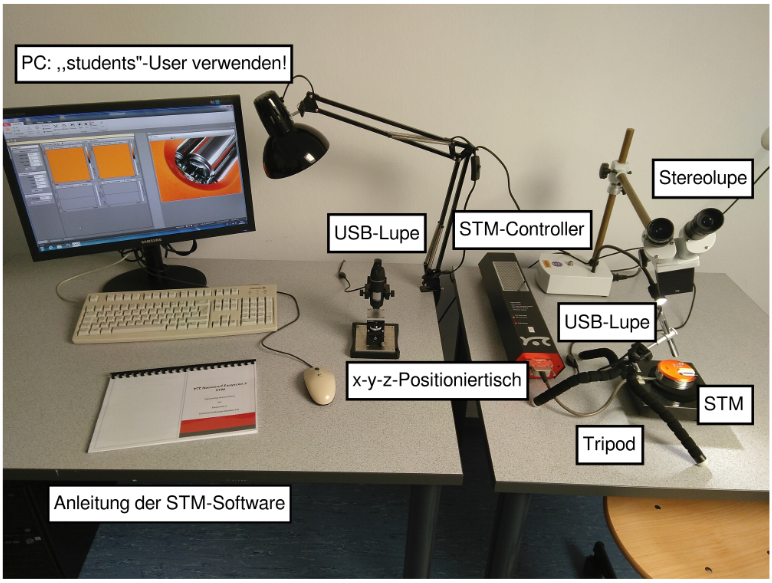
\includegraphics[width=.5\textwidth]{422_aufbau.png}
  \caption{Experimentiertisch.\cite{anleitung422}} \label{fig:aufbau}
\end{figure}
Das STM ist in Abb.\ (\ref{fig:naiostm}) zu sehen.
Der silberne Zylinder ist der Probenhalter, an dem die Probe mit einem Magneten festgehalten wird.
Der Probenhalter wird mit dem Slip--Stick Mechanismus bewegt.
Gegenüber der Probe ist eine Klammer, die einen Pt--Ir Draht hält (Abb.\ (\ref{fig:naiostm_closeup})).
Dieser ist die Spitze des Mikroskops.
Siehe auch Abb.\ (\ref{fig:spitze1}) und (\ref{fig:spitze2}).
\begin{figure}[t]
  \centering
  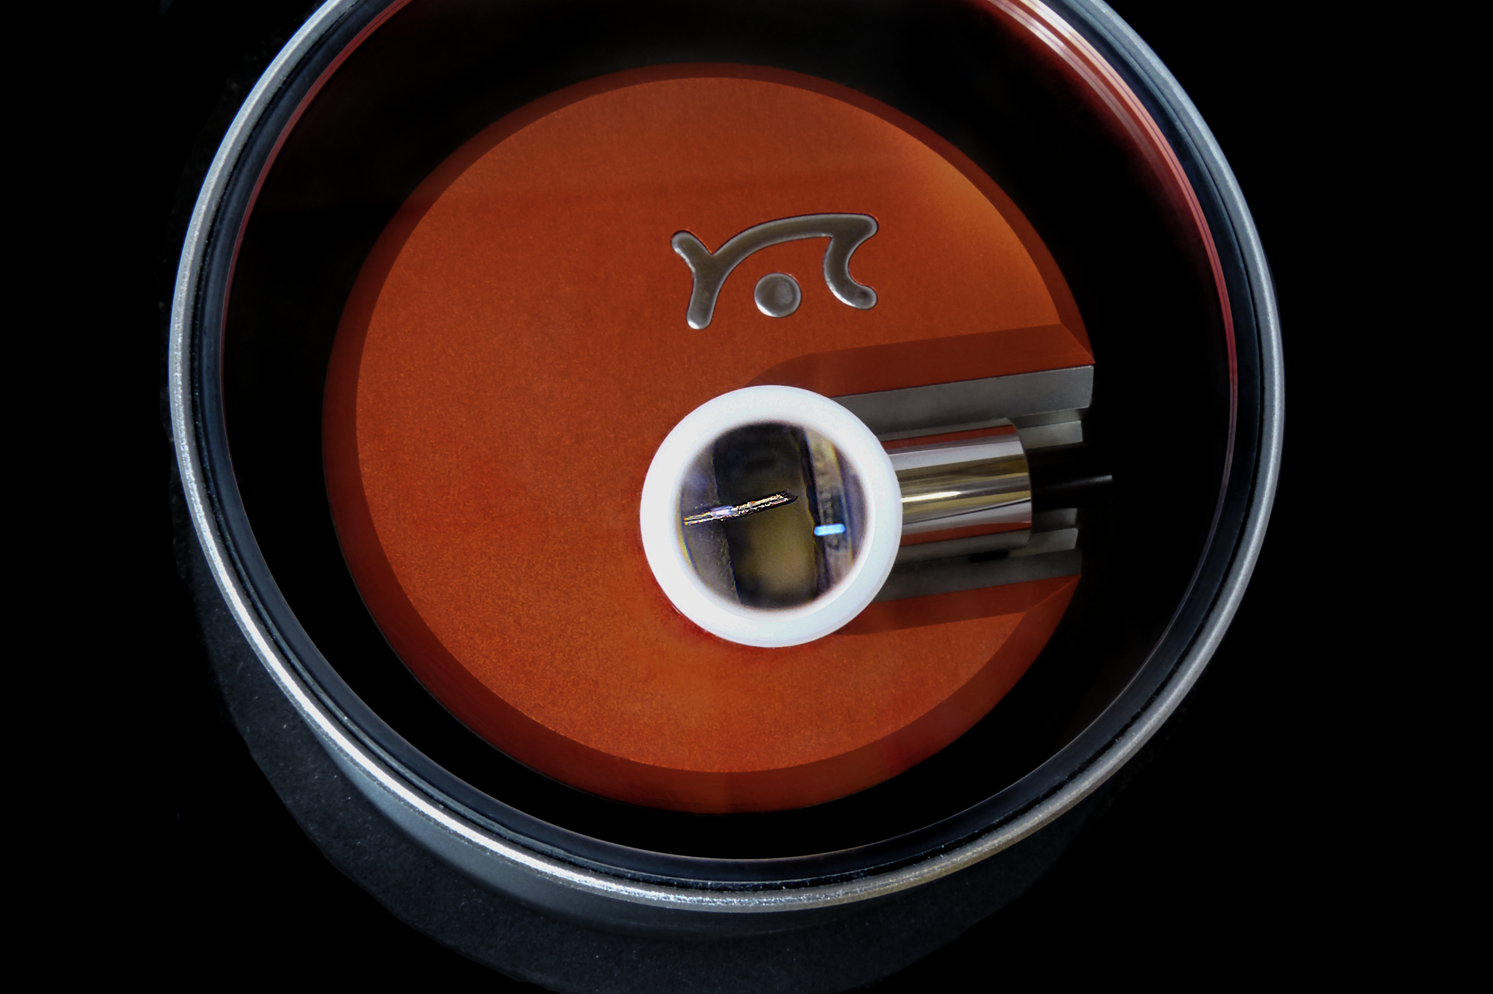
\includegraphics[width=.5\textwidth]{422_naiostm.png}
  \caption{NaioSTM von Nanosurf.\cite{nanosurf}} \label{fig:naiostm}
\end{figure}
\begin{figure}[t]
  \centering
  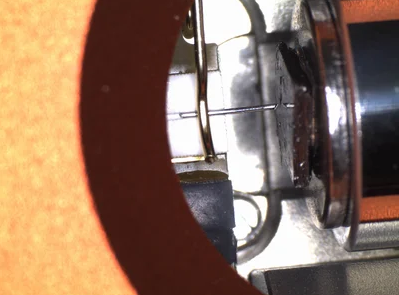
\includegraphics[width=.5\textwidth]{422_naiostm_closeup.png}
  \caption{NaioSTM von Nanosurf, Nahaufnahme der Spitze und Probe.\cite{nanosurf}} \label{fig:naiostm_closeup}
\end{figure}
\subsection{Theoretischer Hintergrund: STM}
Werden Spitze und Probe nah genug aneinander gefahren (s. Abb.\ (\ref{fig:naiostm_closeup})\footnote{Während der Messung sind Spitze und Probe in einem Abstand von wenigen zehntel Nanometer.}), so ist es den Elektronen im \textsc{Fermi}--Niveau der Probe möglich zur Spitze zu tunneln.
Dadurch entsteht ein Tunnelstrom.
Ein Bild der Probe wird erzeugt, in dem der gemessene Strom gegen den Ort aufgetragen wird.
Dieses Bild wird mit der \glqq Easyscan 2\grqq{} Software von Nanosurf aufgenommen.

Die Spitze kann mit makroskopischen Methoden von einem langen Pt--Ir Draht gewonnen werden.
Dabei wird ein kleines Stück des Drahtes mit einer Zange abgerissen, wodurch sich eine mikroskopisch kleine Spitze bildet.
Da die Spitze nicht zu allen Seiten streng monoton fallend sein muss, sondern ausreichend ist, wenn es nur eine Stelle gibt, die der Probe am nächsten ist, kann diese Methode gut verwendet werden.

Die Probe wird mit dem Slip--Stick Mechanismus an die Spitze herangefahren.
Dabei wird der Probenhalter mit einem anderen Material (z.B.\ Gummi) in Kontakt gebracht.
Da der Haftreibungskoeffizient größer als der Gleitreibungskoeffizient ist, kann durch langsame Bewegung des Gummis die Haftung zum Probenhalter erhalten bleiben und der Probenhalter wird verschoben.
Durch schnelles Zurückziehen des Gummis gleitet dies über den Probenhalter zurück in seine ursprüngliche Position und kann erneut am Probenhalter haften.

Die Bewegung der Probe orthogonal zur Spitze werden mit Hifle von \textsc{Piezo}--Kristallen realisiert.
Ein \textsc{Piezo}--Kristall besitzt in einer bestimmten Achse des Gitters keine Spiegelsymmetrie, wodurch mechanische Stauchung und Streckung eine Potentialdifferenz im Kristall verursachen.
Dieses Phänomen funktioniert auch andersherum.
Druch eine angelegte Spannung verschieben sich die Ladungsträger, wodurch eine Stauchung oder Streckung verursacht wird.
Dadruch wird die Probe (der Probenhalter) orthogonal verschoben.

Das STM kann in zwei Modi verwendet werden.

Im \textit{constant current mode} wird die Entfernung der Spitze von der Probe so reguliert, dass immer die gleiche Stromstärke gemessen wird.
Dies wird mit einem PID--Regelkreis (proportional integral differential) realisiert.
Die Einstellung hierfür sind $P=2000$, $I=2000$ und $D=0$.
Dieser Modus ist vor Allem für Proben mit unebenem Höhenprofil vorteilhaft, um die Spitze nicht auf der Probe auflaufen zu lassen.

Im \textit{constant height mode} wird die Entfernung der Spitze von der Probe konstant gelassen.
Dies ermöglicht eine wesentlich schnellere Messung, ist allerdings nur für ebene Proben ratsam.
Die Einstellung des PID--Regelkreises sind $P=0$, $I=4$ und $D=0$.

\section{Durchführung \& Auswertung:\\Goldprobe}

\section{Durchführung \& Auswertung:\\HOPG--Probe}

\section{Fazit}

\bibliography{refs}

\clearpage
\section{Appendix}
\begin{figure}[h]
  \centering
  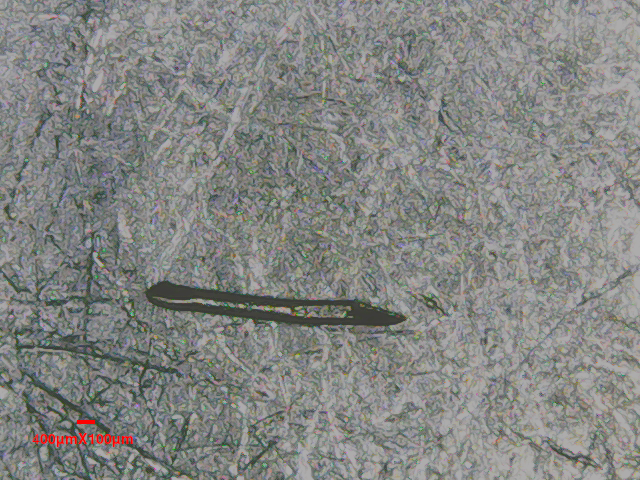
\includegraphics[width=.5\textwidth]{../data/Spitze1_1.png}
  \caption{Spitze 1.} \label{fig:spitze1}
\end{figure}
\begin{figure}[h]
  \centering
  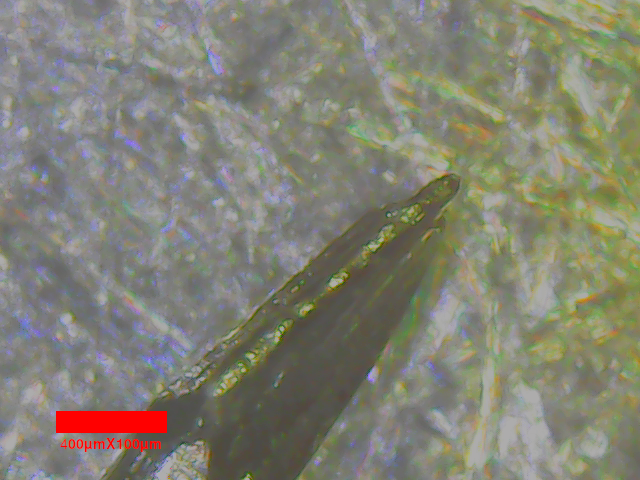
\includegraphics[width=.5\textwidth]{../data/Spitze1_2.png}
  \caption{Spitze 2.} \label{fig:spitze2}
\end{figure}
\clearpage
\begin{figure}[t]
  \centering
  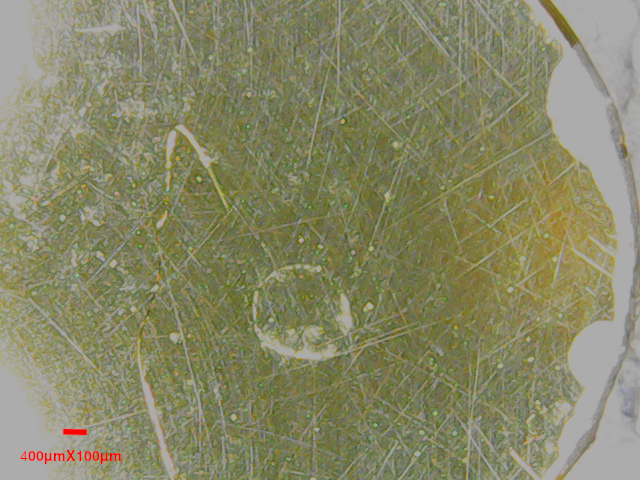
\includegraphics[width=.5\textwidth]{../data/Gold_1.png}
  \caption{Gold fern.}
\end{figure}
\begin{figure}[t]
  \centering
  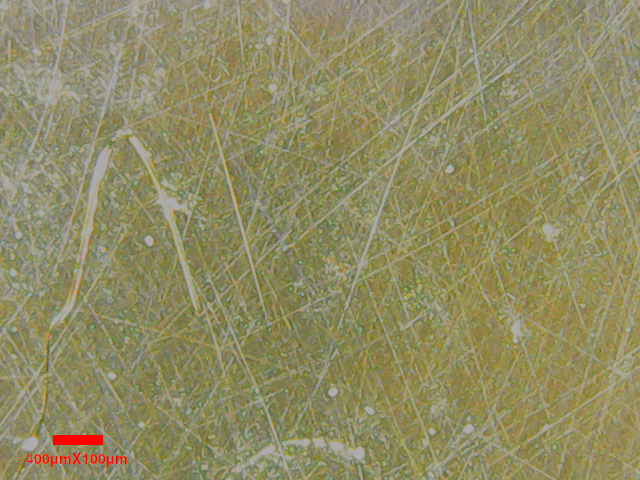
\includegraphics[width=.5\textwidth]{../data/Gold_2.png}
  \caption{Gold mittel.}
\end{figure}
\begin{figure}[t]
  \centering
  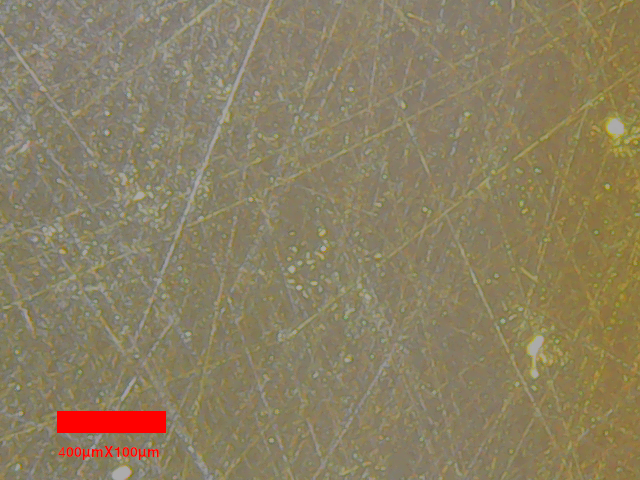
\includegraphics[width=.5\textwidth]{../data/Gold_3.png}
  \caption{Gold nah.}
\end{figure}
\begin{figure}[t]
  \centering
  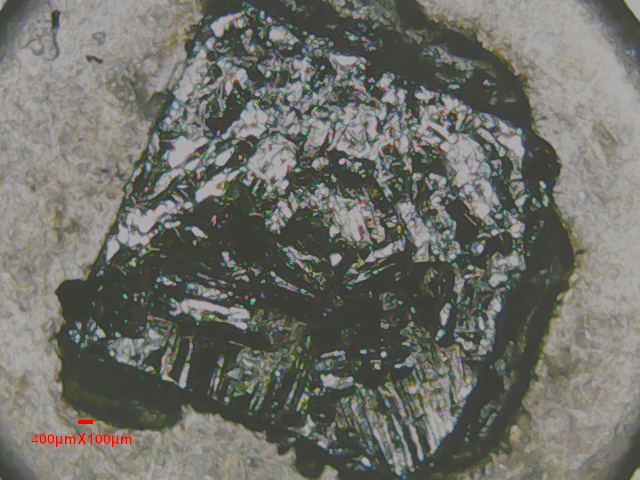
\includegraphics[width=.5\textwidth]{../data/Graphit_3.png}
  \caption{Graphit fern.}
\end{figure}
\begin{figure}[t]
  \centering
  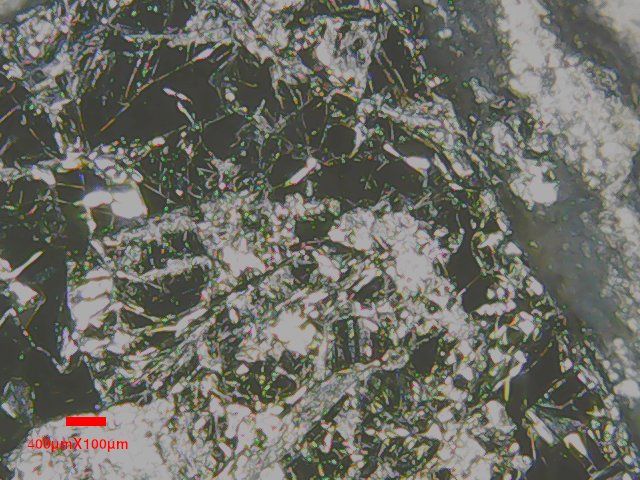
\includegraphics[width=.5\textwidth]{../data/Graphit_1.png}
  \caption{Graphit mittel.}
\end{figure}
\begin{figure}[t]
  \centering
  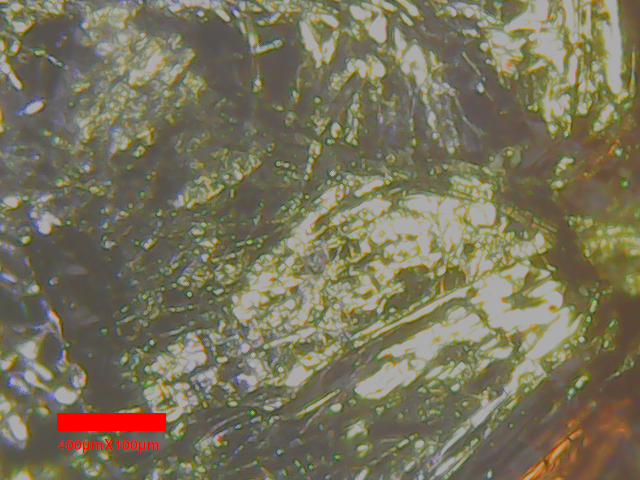
\includegraphics[width=.5\textwidth]{../data/Graphit_2.png}
  \caption{Graphit nah.}
\end{figure}

% TODO: Grobe aufteilung. Kann immer geändert werden. Ist jetzt nicht so festgelegt. Nur als Orientierung.
\section{Spitzen}
\section{Gold Probe}
\begin{figure}[t]
        \centering
        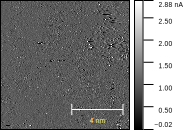
\includegraphics[width=.5\textwidth]{../data/Gold_10nm_current.png}
        \caption{Gold: Strom Karte bei const. current Modus (Setpoint=\SI{1}{\nano A}, P-Gain=\SI{1000}{}, I-Gain=\SI{2000}{} und Tip voltage=\SI{1}{V})} \label{fig:g10nmc}
\end{figure}
\begin{figure}[t]
        \centering
        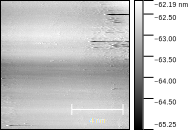
\includegraphics[width=.5\textwidth]{../data/Gold_10nm_z.png}
        \caption{Gold: Höhen Karte bei const. current Modus (Setpoint=\SI{1}{\nano A}, P-Gain=\SI{1000}{}, I-Gain=\SI{2000}{} und Tip voltage=\SI{1}{V})} \label{fig:g10nmz}
\end{figure}
\begin{figure}[t]
        \centering
        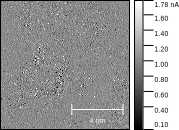
\includegraphics[width=.5\textwidth]{../data/Gold_10nm_50mV_current.png}
        \caption{Gold: Strom Karte bei const. current Modus (Setpoint=\SI{1}{\nano A}, P-Gain=\SI{1000}{}, I-Gain=\SI{2000}{} und Tip voltage=\SI{50}{\milli V})} \label{fig:g10nm50mVc}
\end{figure}
\begin{figure}[t]
        \centering
        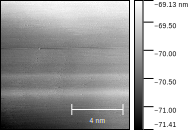
\includegraphics[width=.5\textwidth]{../data/Gold_10nm_50mV_z.png}
        \caption{Gold: Höhen Karte bei const. current Modus (Setpoint=\SI{1}{\nano A}, P-Gain=\SI{1000}{}, I-Gain=\SI{2000}{} und Tip voltage=\SI{50}{\milli V})} \label{fig:g10nm50mVz}
\end{figure}
\begin{figure}[t]
        \centering
        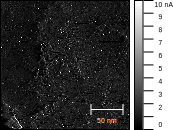
\includegraphics[width=.5\textwidth]{../data/Gold_200nm_current.png}
        \caption{Gold: Strom Karte bei const. current Modus (Setpoint=\SI{1}{\nano A}, P-Gain=\SI{1000}{}, I-Gain=\SI{2000}{} und Tip voltage=\SI{1}{V})} \label{fig:g200nmc}
\end{figure}
\begin{figure}[t]
        \centering
        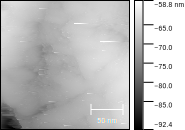
\includegraphics[width=.5\textwidth]{../data/Gold_200nm_z.png}
        \caption{Gold: Höhen Karte bei const. current Modus (Setpoint=\SI{1}{\nano A}, P-Gain=\SI{1000}{}, I-Gain=\SI{2000}{} und Tip voltage=\SI{1}{V})} \label{fig:g200nmz}
\end{figure}
\begin{figure}[t]
        \centering
        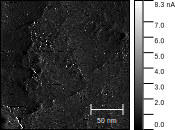
\includegraphics[width=.5\textwidth]{../data/Gold_200nm_50mV_current.png}
        \caption{Gold: Strom Karte bei const. current Modus (Setpoint=\SI{1}{\nano A}, P-Gain=\SI{1000}{}, I-Gain=\SI{2000}{} und Tip voltage=\SI{50}{\milli V})} \label{fig:g200nm50mVc}
\end{figure}
\begin{figure}[t]
        \centering
        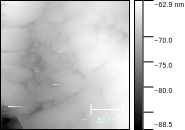
\includegraphics[width=.5\textwidth]{../data/Gold_200nm_50mV_z.png}
        \caption{Gold: Höhen Karte bei const. current Modus (Setpoint=\SI{1}{\nano A}, P-Gain=\SI{1000}{}, I-Gain=\SI{2000}{} und Tip voltage=\SI{50}{\milli V})} \label{fig:g200nm50mVz}
\end{figure}
\begin{figure}[t]
        \centering
        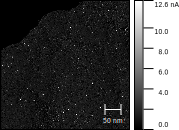
\includegraphics[width=.5\textwidth]{../data/Gold_400nm_current.png}
        \caption{Gold: Strom Karte bei const. current Modus (Setpoint=\SI{1}{\nano A}, P-Gain=\SI{1000}{}, I-Gain=\SI{2000}{} und Tip voltage=\SI{1}{V})} \label{fig:g400nmc}
\end{figure}
\begin{figure}[t]
        \centering
        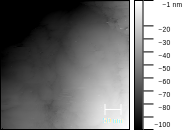
\includegraphics[width=.5\textwidth]{../data/Gold_400nm_z.png}
        \caption{Gold: Höhen Karte bei const. current Modus (Setpoint=\SI{1}{\nano A}, P-Gain=\SI{1000}{}, I-Gain=\SI{2000}{} und Tip voltage=\SI{1}{V})} \label{fig:g400nmz}
\end{figure}
\section{Graphit Probe}
% TODO: Beachte, dass die beiden pngs hier mit 1V benannte sind, aber eigentlich 50mV Tip voltage hatten
\begin{figure}[t]
        \centering
        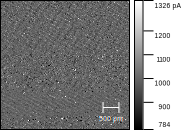
\includegraphics[width=.5\textwidth]{../data/Graphit_4nm_1V_current.png}
        \caption{Gold: Strom Karte bei const. current Modus (Setpoint=\SI{1}{\nano A}, P-Gain=\SI{1000}{}, I-Gain=\SI{2000}{} und Tip voltage=\SI{50}{\nano V})} \label{fig:gr4nm50mVc}
\end{figure}
\begin{figure}[t]
        \centering
        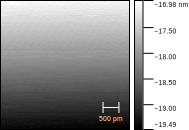
\includegraphics[width=.5\textwidth]{../data/Graphit_4nm_1V_z.png}
        \caption{Gold: Höhen Karte bei const. current Modus (Setpoint=\SI{1}{\nano A}, P-Gain=\SI{1000}{}, I-Gain=\SI{2000}{} und Tip voltage=\SI{50}{\nano V})} \label{fig:gr4nm50mVz}
\end{figure}
\end{document}
